\section{Notation and Preliminaries}\label{s:prel}

In what follows, we let $G=(V,E)$ be a \emph{directed} graph, whose edges $(u,v) \in E$ carry a
binary label $\yuv\in \spin$. The edge labeling will sometimes be collectively denoted by the
$|V|\times |V|$ matrix $Y = [\yuv]$, where $\yuv = \yuv$ if $(u,v) \in E$, and $\yuv = 0$,
otherwise. The corresponding edge-labeled graph will be denoted by $G(Y) = (V,E(Y))$. We use
$\Nin(u)$ and $\Nout(u)$ to denote, respectively, the set of edges incoming to and outgoing from
node $u \in V$, with $\din(u) = \big|\Nin(u)\big|$ and $\dout(u) = \big|\Nout(u)\big|$ being the
in-degree and the out-degree of $u$. Moreover, $\din^+(u)$ is the number of edges $(k,u)\in\Nin(u)$
such that $y_{k,u} = +1$. We define $\din^-(u)$, $\dout^+(u)$, and $\dout^-(u)$ similarly, so that,
for instance, $\dout^-(u)/\dout(u)$ is the fraction of outgoing edges from node $u$ whose label in
$G(Y)$ is $-1$. We call $tr(u) = \dout^-(u)/\dout(u)$ the \emph{trollness} of node $u$, and $un(u)
= \din^-(u)/\din(u)$ the \emph{untrustworthiness} of node $u$. Finally, we also use the notation
$\NNin(u)$ and $\NNout(u)$ to represent, respectively, the in-neighborhood and the out-neighborhood
of node $u \in V$.

Given the directed graph $G = (V,E)$, we define two \emph{edge-to-node reductions} transforming the
original graph $G$ into other graphs. As we see later, these reductions are useful in turning the
edge sign prediction problem into a \emph{node} sign prediction problem (often called node
classification problem), for which many algorithms are indeed available~%
\autocites{BC01}{LabelPropa03}{BDL06}{HP07}{HLP09}{Vitale2012}{HPV12}{WTA13}{HPG15}.  Although any
node classification method could in principle be used, the reductions we describe next are
essentially aimed at preparing the ground for quadratic energy-minimization approaches computed
through a \emph{Label Propagation} algorithm~\autocites{LabelPropa03}{BDL06}.

The first reduction, called $G \rightarrow G'$, builds an \emph{undirected} graph $G' = (V',E')$ as
follows. Each node $u \in V$ has two copies in $V'$, call them $\iin$ and $\iout$. Each directed
edge $(u,v)$ in $E$ is associated with one node, call it $e_{u,v}$, in $V'$, along with the two
undirected edges $(\iout,e_{u,v})$ and $(e_{u,v},\jin)$. Hence $|V'| = 2|V|+|E|$ and $|E'| = 2|E|$.
Moreover, if $G = G(Y)$ is edge labeled, then this labeling transfers to the subset of nodes
$e_{u,v} \in V'$, so that $G'$ is a graph $G'(Y) = (V'(Y),E')$ with partially-labeled nodes. The
second reduction, called $G \rightarrow G''$, builds an \emph{undirected and weighted} graph $G'' =
(V'',E'')$. Specifically, we have $V'' \equiv V'$ and $E'' \supset E'$, where the set $E''$ also
includes edges $(\iout,\jin)$ for all $u$ and $v$ such that $(u,v) \in E$. The edges in $E'$ have
weight $2$, whereas the edges in $E''\setminus E'$ have weight $-1$. We provide in
\autoref{ssec:troll_lprop_weights} an analytic justification for this weights choice in the context
of Label Propagation. Finally, as in the $G \rightarrow G'$ reduction, if $G = G(Y)$ is edge
labeled, then this labeling transfers to the subset of nodes $e_{u,v} \in V''$. Graph $G'$, which
will not be used in this paper, is an intermediate structure between $G$ and $G''$ and provides a
conceptual link to the standard cutsize measure in node sign classification. \autoref{f:etnr}
illustrates these two reductions. 

\begin{figure*}[t]
  \centering
  \begin{subfigure}[b]{0.28\textwidth}
    \centering 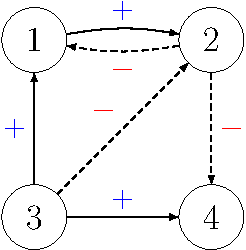
\includegraphics[height=.10\textheight]{g_latex-crop} \caption{}
  \end{subfigure}~
  \begin{subfigure}[b]{0.30\textwidth}
    \centering 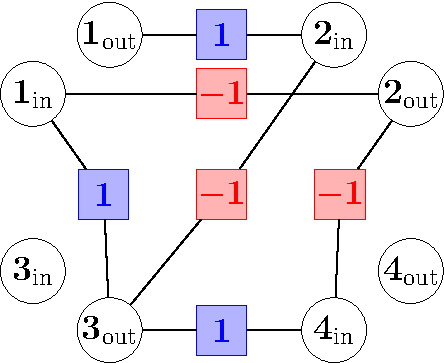
\includegraphics[height=.12\textheight]{gprime_latex-crop}
    \caption{\label{fig:troll_reduction_gprime}}
  \end{subfigure}~
  \begin{subfigure}[b]{0.36\textwidth}
    \centering 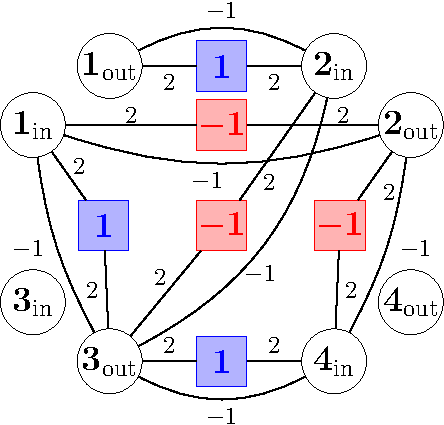
\includegraphics[height=.14\textheight]{gsecond_latex-crop} \caption{}
  \end{subfigure}
  \caption{\label{f:etnr}
    \textbf{(a)} A directed edge-labeled graph $G$. \textbf{(b)} Its corresponding graph $G'$
    resulting from the $G\rightarrow G'$ reduction. The square nodes in $G'$ correspond to the
    edges in $G$, and carry the same labels as their corresponding edges. On the other hand, the
    $2|V|$ circle nodes in $G'$ are unlabeled. Observe that some nodes in $G'$ are isolated and
    thus unimportant. These are exactly the nodes in $G'$ corresponding to the nodes having in $G$
    no outgoing or no incoming edges: for instance nodes $3$ and $4$ in $G$. \textbf{(c)} The
    weighted graph resulting from the $G\rightarrow G''$ reduction.
  }
\end{figure*}

These reductions are meaningful only if they are able to approximately preserve label
\emph{regularity} when moving from edges to nodes. That is, if the edge sign prediction problem is
easy for a given $G(Y) = (V,E(Y))$, then the corresponding node sign prediction problems on $G'(Y)
= (V'(Y),E')$ and $G''(Y) = (V''(Y),E)$ are also easy, and vice versa.  While we could make this
argument more quantitative, here we simply observe that if each node in $G$ tends to be either
troll or trustworthy, then few labels from the incoming and outgoing edges of each such node are
sufficient to predict the labels on the remaining edges in $G$, and this translates to a small
cutsize\footnote{Recall that the cutsize of an undirected node-labeled graph $G'(Y)$ is the number
of edges in $G'$ connecting nodes having mismatching labels.} of $G'(Y)$ over the nodes
corresponding to the edges in $G$ (the colored squares in \autoref{fig:troll_reduction_gprime}).

Again, we would like to point out that these reductions serve two purposes: First, they allow us to
use the many algorithms designed for the better studied problem of node sign prediction. Second,
the reduction $G\rightarrow G''$ with the specific choice of edge weights is designed to make the
Label Propagation solution approximate the maximum likelihood estimator associated with our
generative model (see Section~\ref{ss:passive}). Note also that efficient Label Propagation
implementations exist that can leverage the sparsity of $G''$.

We consider two learning settings associated with the problem of edge sign prediction: a batch
setting and an online setting. In the batch \emph{passive} setting, we assume that a training set
of edges $E_0$ has been drawn uniformly at random \emph{without replacement} from $E$, we observe
the labels in $E_0$, and we are interested in predicting the sign of the remaining edges $E
\setminus E_0$ by making as few prediction mistakes as possible. In the batch \emph{active}
setting, we are given a budget of edge labels to observe, and are free to select them the way we
want within $E(Y)$. Again, the goal is to make as few mistakes as possible on the remaining edges.
The specific batch setting (passive and active) we study here assumes that labels are produced by a
generative model which we describe in the next section, and our label regularity measure is a
quadratic function (denoted by $\Psi^2_{G''}(Y)$ and defined in \autoref{s:exp}), related to this
model. $\Psi^2_{G''}(Y)$ is small just when all nodes in $G$ tend to be either troll or
trustworthy. 

On the other hand, the \emph{online} setting we consider is the standard mistake bound model of
online learning~\autocite{Winnow88} where all edge labels are assumed to be generated by an
adversary and sequentially presented to the learner according to an arbitrary permutation. For an
online learning algorithm $A$, we are interested in measuring the total number of mistakes $M_A(Y)$
the algorithm makes over $G(Y)$ when the worst possible presentation order of the edge labels in
$Y$ is selected by the adversary.

\iffalse
  In this setting, learning is split into a sequence of rounds: At each round $t=1,2,\dots$ a
  learning algorithm $A$ outputs a prediction ${\wh y_t} \in \spin$ for the label $y_t \in \spin$
  of an edge arbitrarily selected by the adversary. After the prediction is made, label $y_t$ is
  revealed to the algorithm, hence allowing it to change its internal state. In the next round a
  new edge is selected by the adversary, and so on. Notice that since the underlying labeling over
  the edges is decided by the adversary once and for all,\footnote{For simplicity, we assume the
  adversary is deterministic.} all edges occur exactly once within the sequence to be predicted (so
  that this game lasts exactly $|E|$ rounds). The adversary decides both the underlying labeling
  $Y$ over the edges of $G$ and the order of their presentation to the learning algorithm. We say
  that $A$ has made a mistake at time $t$ if ${\wh y_t} \neq y_t$, and we measure $A$'s prediction
  performance simply through the total number of mistakes $M_A(Y)$ it makes over $G(Y)$ when the
  worst possible presentation order of the edge labels in $Y$ is selected by the adversary. As is
  standard, we contrast $M_A(Y)$ to some kind of \emph{regularity} measure $\Psi_G(Y)$ of the
  labeling $Y$ over $G$, so that we are in fact aimed at bounding the (cumulative) regret \( M_A(Y)
  - \Psi_G(Y)~.\)
\fi

Also in the online setting our label regularity measure, denoted here by $\Psi_G(Y)$, is small when
nodes in $G$ tend to be either troll or trustworthy. When this happens, few labels from the
incoming and outgoing edges of each node are sufficient to predict the labels on the remaining
edges. Formally, for fixed $G$ and $Y$, let 
$$
\Psiin(v,Y) = \min\big\{\din^-(v),\din^+(v)\big\}
\qquad\text{and}\qquad
\Psiout(u,Y) = \min\big\{\dout^-(u),\dout^+(u)\big\}
$$
Let also
$$
\Psiin(Y) = \sum_{v \in V} \Psiin(v,Y)
\qquad\text{and}\qquad
\Psiout(Y) = \sum_{u \in V} \Psiout(u,Y)
$$
Then we define $\Psi_G(Y) = \min\big\{\Psiin(Y),\Psiout(Y)\big\}$. The two measures
$\Psi^2_{G''}(Y)$ and $\Psi_G(Y)$ are conceptually related and their value on real data is quite
similar (see \autoref{tab:all_mcc} in \autoref{s:exp}).

\iffalse
  Recall that the cutsize of an undirected node-labeled graph $G'(Y)$ is the number of edges in
  $G'$ connecting nodes having mismatching labels. Now, because the only nodes in $G'$ we are
  interested in predicting are those corresponding to the edges in $G$ (the colored squares in
  Figure \ref{f:etnr} (b)), the online prediction problem on the edges of $G$ translates to a node
  sign prediction problem on a subset of $V'$. The remaining nodes in $V'$ (the circles in Figure
  \ref{f:etnr} (b)) we are free to assign dummy labels so as to minimize the corresponding mistake
  bound over $G'$. It is straightforward to see that if we set the labeling $Y$ on $V'$ in such a
  way that $y_{\iout} = +1$ if $tr(u) < 0$, and $-1$, otherwise, and $y_{\iin} = +1$ if $un(u) <
  0$, and $-1$, otherwise, then the cutsize of $G'(Y)$ equals\footnote{In fact, for the sake of
  this specific argument, nothing prevents from retaining of $G'$ either only the edges
  $(\iout,e_{u,v})$ or only the edges $(e_{u,v},\jin)$, resulting in a cutsize of $\Psiout(Y)$ and
  $\Psiin(Y)$, respectively.} $\Psiin(Y) + \Psiout(Y)$.
\fi
